\documentclass[12pt,letterpaper]{extarticle}

\usepackage{caption} % for the figure captions
\usepackage[osf]{mathpazo} % a nicer font
% this is a package for the citation formats: found this formulation sorted natbib errors when changing packages
%from http://tex.stackexchange.com/questions/54480/package-natbib-error-bibliography-not-compatible-with-author-year-citations
\usepackage[square,sort,comma,numbers]{natbib} 
\usepackage{amsmath} % package for equations
\usepackage{url} % package for urls
\usepackage{hyperref} % for hyperlinks
\usepackage[a4paper, total={6in, 9in}]{geometry}
\hypersetup{
     colorlinks   = true,
     citecolor    = gray
}
\usepackage{graphicx} % for the figures
\usepackage{pdfpages}
\hypersetup{linkcolor=blue}

\pagenumbering{gobble}

\graphicspath{ }

%Title page
%Itinerary
%Localities
%Kit list
%Contact details
%Where staying: all deets

\begin{document}

%title

{\Huge\textbf{\textit{Mesacanthus}}\par}
\vspace{3mm}
{\large{me-sa-can-thus} \par} 
\vspace{5mm}
\textit{Mesacanthus} is a \textbf{``spiny shark''}, or acanthodian fish, from Scotland, with bony spines in front of each fin and tiny, shark-like scales.  It was one of the \textbf{earliest relatives of living sharks}, and like all of our fishes it lived in the \textbf{Devonian} period, between 420 and 360 million years ago.  It had no teeth, and instead would have fed by \textbf{filtering plankton} out of the water with its sieve-like gills.  \textit{Mesacanthus} was one of the \textbf{smallest} acanthodians (2-15cm) and would have been eaten by bigger fishes, including other spiny sharks like \textit{Ischnacanthus} - the coprolite (fossil poo) on the table is probably mainly made up of lots of tiny digested \textit{Mesacanthus}.\newline

\begin{figure}[h!]
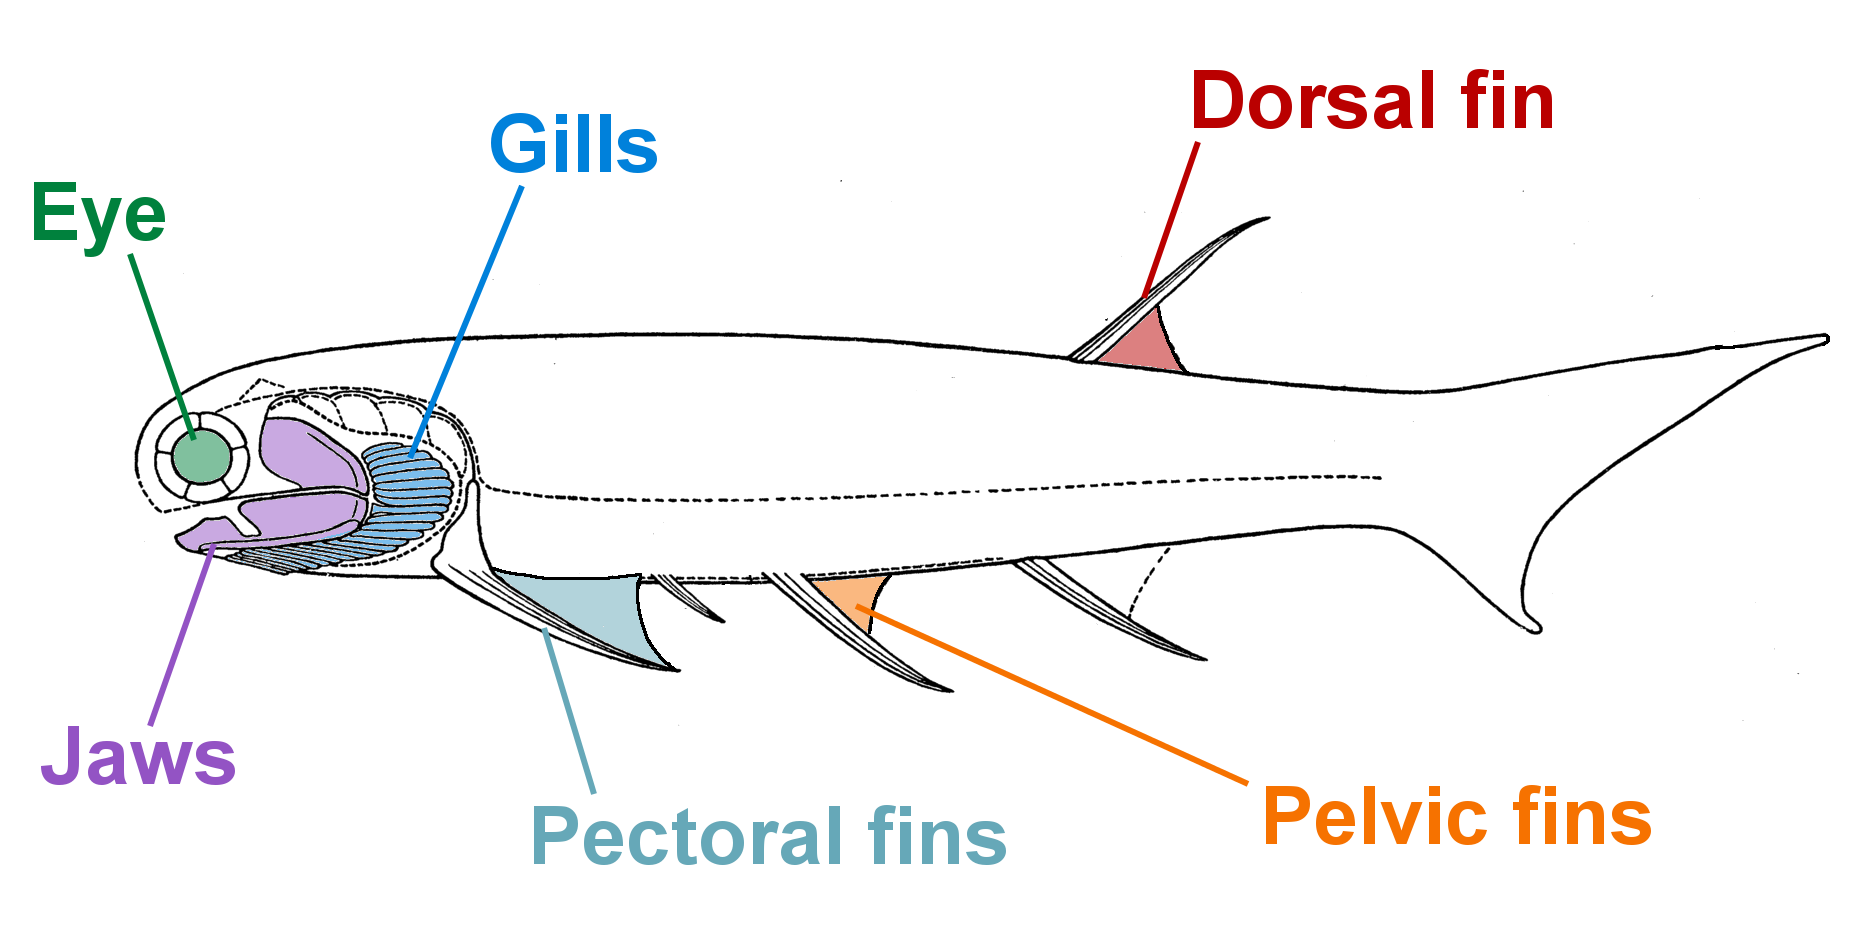
\includegraphics[scale=0.5]{Mesacanthus}
\centering
\end{figure}

{\large\textbf{\underline{Fossil facts}}\par}

\begin{itemize}
  \item We have \textit{Mesacanthus} from \textbf{two different places} in Scotland: Tillywhandland Quarry near Dundee, and Achanarras Quarry near Thurso.  You can tell this from the different colours of the rock they're in.
  \item As you can see \textit{Mesacanthus} was \textbf{really small in comparison to some of the other fishes of the time} (look at our smallest one!).  It probably had a role in the ecosystem similar to small, filter-feeding fishes today, unlike living sharks which are all quite big (can you think of any goldfish sized sharks?).
\end{itemize}


\end{document}